\chapter{Einleitung}
\section{Ausgangslage}
{\projectpartner} ist ein Unternehmen mit Sitz in Leonding, das sich auf Innenarchitektur und Glasdekore spezialisiert hat, die verschiedenste Räumlichkeiten wie Bars, Hotelzimmer und etc. für den Kunden attraktiver machen. SanMod-Bäder bieten individuelle, freistehende Sanitärmodule für einen flexiblen und zeitsparenden Einbau in Gebäuden. Zurzeit werden die Bäder dem Kunden mit einem Video präsentiert. Diese Methode bringt aber Nachteile mit sich da die Bäder immer nur aus einer Perspektive gezeigt werden, die Modelle unflexibel sind, nicht interaktiv und Kundenwünsche nicht sofort umgesetzt werden können. Diese Probleme werden durch die Applikation behoben und macht es möglich die Designentwürfe für spätere Zwecke abzuspeichern.

\section{Zielsetzung}
Das Ziel ist es die Planung zu erleichtern und gegebenenfalls Änderungen sofort im Kundengespräch umzusetzen. Durch diese virtuelle Stütze können sich alle Beteiligten das fertige Bad besser vorstellen, und mögliche Missverständnisse sofort klären. Kundengespräche werden dadurch aufgewertet und effizienter.

\section{Aufbau der Diplomarbeit}
Die Diplomarbeit ist in drei Teile gegliedert. 
Der erste Teil besteht aus den verwendeten Technologien.
Der zweite Teil geht näher auf die Grundlagen und Methoden der Arbeit ein.
Der dritte und letzte Teil behandelt die Umsetzung und Realisierung des Projektes.
Außerdem wird hier auf die Systemarchitektur eingegangen und die Implementierung so wie
der Release der Diplomarbeit.


\begin{figure}
\begin{center}
	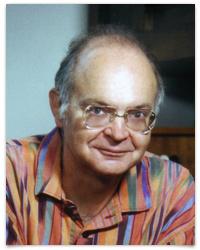
\includegraphics[scale=.5]{images/don_knuth.jpg}
\end{center}
	\caption{Don Knuth, the inventor of \TeX}
	\label{fig:sample}
\end{figure}

\section{Basic Terminology}
As usual the very basic terminology is briefly explained here. Most probably the explanations here only scratch a surface level. More detailed explanations of terminology goes into chapter%~\ref{cha:theoretical-background}.

\section{Related Work and Projects}
Here a survey of other work in and around the area of the thesis is given. The reader shall see that the authors of the thesis know their field well and understand the developments there. Furthermore here is a good place to show what relevance the thesis in its field has.

\section{Structure of the Thesis}
%dsflkjas flaksjfl asdfj as lfjldsajflaksdjf sa dfjlasdkfj sadlfjasdklf als dfj l dfsdfsdfn chapter~\ref{cha:used-technologies} (\nameref{cha:used-technologies}) on page~\pageref{cha:used-technologies} we describe the used technologies.
Finally the reader is given a brief description what (s)he can expect in the thesis. Each chapter is introduced with a paragraph roughly describing its content.